\section{Anatomy of the Basal Ganglia}
\label{intro:BGAnatomy}
The \gls{bg} are a set of interconnected subcortical nuclei.
Their neural organization is highly preserved in vertebrates for over 500 million years~\cite{Grillner2016BG}.
The \gls{bg} may be viewed as a two-input two-output system.
The striatum and the \gls{stn} are the input structures receiving excitatory afferents from virtually the entire cerebral cortex and thalamus.
The output nuclei are the internal segment of the globus pallidus, also called \gls{gpi}, and the \gls{snr}.
The output structures receive inhibitory input from the striatum and excitatory input from the \gls{stn}.
They both contain tonically-active GABAergic neurons that target motor centers in the brainstem and thalamus.
There are no direct connections from the \gls{bg} outputs to motor neurons of the brainstem or spinal cord~\cite{Mink1996}.
\par
Other than the input and output nuclei, the \gls{bg} also include \emph{intrinsic} structures:
The external segment of the globus pallidus, called \gls{gpe}, is also innervated by the striatum as well as the \gls{stn} and projects back to the \gls{stn} and the output nuclei.
\Gls{snc} is the center of \gls{da}-containing neurons in the \gls{bg} and targets the striatal neurons.
\autoref{fig:intro:BGAnatomy} summarizes the anatomy of the \gls{bg}.

\begin{figure}[bth]
	\begin{center}
		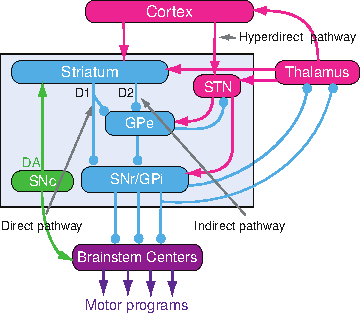
\includegraphics[width=0.7\linewidth]{ch-intro/figures/BGAnatomy}
		\caption[Anatomy of the Basal Ganglia]
		{\textbf{Schematic Anatomy of the basal ganglia.}
		The gray highlighted rectangle depicts the BG nuclei.
		Arrows show anatomical connections (\textit{red}: glutamatergic; \textit{blue}: GABAergic; \textit{green}: DAergic).
		STN:~subthalamic nucleus;
		GPe:~globus pallidus externus;
		SNc:~substantia nigra pars compacta;
		SNr:~substantia nigra pars reticulata;
		GPi:~globus pallidus internus;
		DA:~dopamine.
		Figure slightly modified from~\cite{Grillner2016BG}.
		}
		\label{fig:intro:BGAnatomy}
	\end{center}
\end{figure}
\subsection{Striatum} \label{intro:anatomy:striatum}
%order of material: MSNs > interneurons > I/O > D/ID pathway > dopamine > topography > DLS/DMS
The striatum is the main input nucleus of the \gls{bg} and one of the largest undivided structures in rodent brain atlas.
Despite several cell types, GABAergic \glspl{msn} constitute~90--95\% of its neural population.
Their name stems from their size and the abundance of their dendritic processes~\cite{TURNER2000BasalFunction}.
They are mostly quiescent, except during  motor activity or in response to sensory stimuli~\cite{KandelBook2001}.
\par
The striatum also contains two major types of inhibitory interneurons.
\Glspl{fsi} target \glspl{msn} at the soma level by gap junctions and provide powerful GABAergic synapses to several hundreds of surrounding \glspl{msn}~\cite{Grillner2016BG, Gage2010FSI}.
Although they are scarce, \glspl{fsi} have higher firing rate compared to \glspl{msn} and are capable of delaying action potentials in the neighboring \glspl{msn}~\cite{Wilson2007GABAergicNeostriatum}.
Large cholinergic interneurons are the other type of striatal interneurons.
They have tonic discharge patterns, and in primate, are referred to as \textit{tonically active neurons}.
\Glspl{fsi} and cholinergic interneurons each comprise approximately~1\% of striatal neurons in rodents, nonetheless, they are believed to strongly contribute to the dominance of inhibition in the striatum~\cite{Gage2010FSI}.
In addition to these two, several other types of GABAergic interneurons within the striatum are described as well~\cite{Grillner2016BG}.
\par
Massive excitatory projections from all areas of cortex target striatal \glspl{fsi} as well as \glspl{msn}.
Intralaminar nuclei of the thalamus also provide excitatory input (\autoref{fig:intro:BGAnatomy}).
Altogether, these glutamatergic synapses make up 80\% of all synapses in the striatum~\cite{Wilson2007GABAergicNeostriatum}.
Moreover, \gls{da}ergic afferents from the \gls{snc} are the main source of neuromodulatory influence.
They primarily synapse with principle neurons (\glspl{msn}).
\Gls{da} release modulates \gls{msn} activity differentially.
\par
\Glsentrylongpl{msn} are the only way out of the striatum.
They project to the globus pallidus and substantia nigra.
Based on their neurochemistry and projection patterns, they are divided into two distinct types.
One class expresses \glspl{d1} and projects directly to \gls{gpi}/\gls{snr} neurons, hence they form the so-called~\emph{direct pathway}.
The second kind expresses \glspl{d2} and projects to \gls{gpe}.
This path, in turn, leads to the output nuclei through two routes:~monosynaptic~\gls{gpe}$\rightarrow$output, or bisynaptic~\gls{gpe}$\rightarrow$\gls{stn}$\rightarrow$output projections~\cite{TURNER2000BasalFunction}.
These \glspl{msn} form the \emph{indirect pathway} (\autoref{fig:intro:BGAnatomy}).
Of note, \gls{stn} efferents form the only intrinsic excitatory connections in the basal ganglia, an otherwise inhibition-dominated structure.
\par
\Gls{da} significantly modulates neuronal activity in the striatum.
Axons from \gls{snc} neurons arborize widely in the striatum.
They mainly target the narrow necks connecting the spines to dendritic shafts, whereas cortical inputs mostly terminate on dendritic shafts.
This particular arrangement may be a mechanism by which \gls{da} release modulates cortical input to the \glspl{msn}~\cite{TURNER2000BasalFunction}.